% संपूर्ण मराठी ग्रंथातील प्रकरण 2: संबंध
% हा संपादनयोग्य स्रोतखंड आहे. संकलनासाठी संपूर्ण स्रोतसंग्रहातील
% अक्षररूपे, पूर्वभाग, चिन्हव्याख्या आणि आकृती-स्रोत आवश्यक आहेत.
% मूळ: Open Logic Project; मजकूर आणि रूपांतर CC BY 4.0.
% यंत्रानुवाद, दुरुस्ती आणि तपासणी: OpenAI Codex —
% GPT-5.6 Sol आणि GPT-6 Sol, दोन्ही Ultra effort.
% दुरुस्ती-पुनरावलोकन: GPT-6.1 Sol, Ultra effort.
\chapter{संबंध}\label{sfr:rel::chap}








\section{संच म्हणून संबंध}\label{sfr:rel:set:sec}

\begin{explain}
\ref{sfr:set:imp:sec} मध्ये आपण काही महत्त्वाच्या संचांचा उल्लेख केला:
$\Nat$, $\Int$, $\Rat$, $\Real$. यांपैकी काही संचांतील घटक
यांच्यातील काही लक्षवेधी संबंध तुम्हाला आठवत असतील. उदाहरणार्थ, या प्रत्येक
संचावर एक सर्वमान्य \emph{क्रमसंबंध} असतो. तसेच, प्रत्येक वस्तूचा फक्त
स्वतःशी आणि इतर कशाशीही नसणारा \emph{एकरूप असण्याचा} संबंध असतो. पुढे
आपल्याला आणखी अनेक लक्षवेधी संबंध भेटतील, आणि शक्य संबंध तर त्याहूनही
अधिक आहेत. त्यांचा आढावा घेण्यापूर्वी मात्र, संबंधांकडे एका विशिष्ट प्रकारचे
संच म्हणून पाहता येते, हे आपण दाखवू.

यासाठी \ref{sfr:set:pai:sec} मधील दोन गोष्टी आठवा. प्रथम,
\emph{क्रमित जोडी} ही संकल्पना: $a$ आणि $b$ दिलेले असतील, तर
$\tuple{a, b}$ बनवता येते. येथे घटकांचा क्रम महत्त्वाचा \emph{असतो}.
म्हणून $a \neq b$ असेल, तर $\tuple{a, b} \neq \tuple{b, a}$.
(याची अक्रमित जोड्यांशी, म्हणजे $2$-घटक संचांशी, तुलना करा: तेथे
$\{a, b\}=\{b, a\}$.) दुसरे म्हणजे, \emph{कार्तीय गुणाकार} ही संकल्पना
आठवा: $A$ आणि $B$ हे संच असतील, तर $A \times B$ बनवता येतो. तो
$x \in A$ आणि $y \in B$ असणाऱ्या सर्व $\tuple{x, y}$ जोड्यांचा संच
आहे. विशेषतः, $A^{2}= A \times A$ हा $A$ मधून घेतलेल्या सर्व क्रमित
जोड्यांचा संच आहे.

आता एका संचावरील विशिष्ट संबंध पाहू: नैसर्गिक संख्यांच्या $\Nat$ या
संचावरील $<$-संबंध. $n<m$ असणाऱ्या संख्यांच्या सर्व $\tuple{n, m}$
जोड्यांचा संच विचारात घ्या, म्हणजे,
\[  R=\Setabs{\tuple{n, m}}{n, m \in \Nat \text{ आणि } n<m}.
\]
$n$ ही संख्या $m$ पेक्षा लहान असणे आणि $\tuple{n, m}$ ही जोडी
$R$ ची सदस्य असणे यांचा निकटचा संबंध आहे, तो असा:
\[      n<m\text{ तेव्हा आणि केवळ तेव्हाच }\tuple{n, m} \in R.
\]
खरे तर, कोणतीही माहिती न गमावता $R$ हा संच \emph{म्हणजेच} $\Nat$
वरील $<$-संबंध आहे, असे आपण मानू शकतो.

त्याचप्रमाणे, संख्यांमधील कोणत्याही संबंधासाठी $\Nat^{2}$ चा एक उपसंच
तयार करता येतो. उलट, संख्यांच्या जोड्यांचा कोणताही $S \subseteq \Nat^{2}$
संच दिला असेल, तर त्याला अनुरूप संख्यांमधील एक संबंध असतो: $n$ चा $m$
शी तो संबंध तेव्हा आणि केवळ तेव्हाच असतो, जेव्हा $\tuple{n, m} \in S$.
यावरून पुढील व्याख्या समर्थित होते:
\end{explain}

\begin{defn}[द्विपदी संबंध]
$A$ या संचावरील \emph{द्विपदी संबंध} म्हणजे $A^{2}$ चा एक उपसंच.
$R \subseteq A^{2}$ हा $A$ वरील द्विपदी संबंध असेल आणि $x, y \in A$
असतील, तर $\tuple{x, y} \in R$ यासाठी आपण कधी कधी $Rxy$ (किंवा $xRy$)
असे लिहितो.
\end{defn}

\begin{ex}
  \label{sfr:rel:set:relations}
नैसर्गिक संख्यांच्या जोड्यांचा $\Nat^{2}$ हा संच अशा द्विमितीय सारणीत
मांडता येतो:
\[  \begin{array}{ccccc}
  \mathbf{\tuple{ 0,0 }} & \tuple{ 0,1 } &
    \tuple{ 0,2 } & \tuple{ 0,3 } & \ldots\\
  \tuple{ 1,0 } & \mathbf{\tuple{ 1,1 }} &
    \tuple{ 1,2 } & \tuple{ 1,3 } & \ldots\\
  \tuple{ 2,0 } & \tuple{ 2,1 } &
    \mathbf{\tuple{ 2,2 }} & \tuple{ 2,3 } & \ldots\\
  \tuple{ 3,0 } & \tuple{ 3,1 } & \tuple{ 3,2 } &
    \mathbf{\tuple{ 3,3 }} & \ldots\\
  \vdots & \vdots & \vdots & \vdots & \mathbf{\ddots}
  \end{array}
\]
येथे कर्णावरील नोंदी ठळक केल्या आहेत, कारण त्या जोड्यांचा बनलेला
$\Nat^2$ चा उपसंच, म्हणजे,
\[  \{\tuple{0,0 }, \tuple{ 1,1 }, \tuple{ 2,2 }, \dots\},
  \]
हा \emph{$\Nat$ वरील एकरूपता संबंध} आहे. (एकरूपता संबंध वारंवार वापरला
जातो, म्हणून कोणत्याही $A$ संचासाठी $\Id{A}=\Setabs{\tuple{ x,x }}{x \in
A}$ अशी व्याख्या करू.) कर्णाच्या वर असलेल्या सर्व जोड्यांचा उपसंच, म्हणजे,
\[  L = \{\tuple{ 0,1 },\tuple{ 0,2 },\ldots,\tuple{ 1,2 },
  \tuple{ 1,3 }, \dots, \tuple{ 2,3 },\tuple{ 2,4 },\ldots\},
\]
हा \emph{लहान असण्याचा} संबंध आहे, म्हणजे $Lnm$ तेव्हा आणि केवळ तेव्हाच,
जेव्हा $n<m$. कर्णाच्या खाली असलेल्या जोड्यांचा उपसंच, म्हणजे,
\[  G=\{ \tuple{ 1,0 },\tuple{ 2,0 },\tuple{
    2,1 }, \tuple{ 3,0 },\tuple{ 3,1 },\tuple{ 3,2 }, \dots\},
\]
हा \emph{मोठे असण्याचा} संबंध आहे, म्हणजे $Gnm$ तेव्हा आणि केवळ तेव्हाच,
जेव्हा $n>m$. $L$ आणि $I$ यांचा संयोग $K=L\cup I$ असा लिहू; तो
\emph{लहान किंवा समान असण्याचा} संबंध आहे: $Knm$ तेव्हा आणि केवळ तेव्हाच,
जेव्हा $n \le m$. त्याचप्रमाणे, $H=G \cup I$ हा \emph{मोठे किंवा समान
असण्याचा संबंध} आहे. $L$, $G$, $K$ आणि $H$ हे \emph{क्रम} नावाच्या
विशिष्ट प्रकारचे संबंध आहेत. $L$ आणि $G$ यांचा गुणधर्म असा: कोणत्याही संख्येचा स्वतःशी $L$ किंवा $G$
संबंध नसतो (म्हणजे, सर्व $n$ साठी $Lnn$ आणि $Gnn$ दोन्ही असत्य असतात).
हा गुणधर्म असणाऱ्या संबंधांना \emph{अपरावर्ती} म्हणतात; आणि ते क्रमही
असतील, तर त्यांना \emph{काटेकोर क्रम} म्हणतात.
\end{ex}

\begin{explain}
क्रम आणि एकरूपता हे महत्त्वाचे व स्वाभाविक संबंध असले, तरी आपल्या
व्याख्येनुसार $A^{2}$ चा \emph{कोणताही} उपसंच हा $A$ वरील संबंध असतो,
तो कितीही कृत्रिम किंवा ओढूनताणून बनवलेला वाटला तरीही. विशेषतः,
$\emptyset$ हा कोणत्याही संचावरील संबंध असतो (हा \emph{रिक्त संबंध};
कोणत्याही घटकजोडीमध्ये तो नसतो), आणि $A^{2}$ हाही $A$ वरील संबंध असतो
(प्रत्येक जोडीमध्ये असणारा); त्याला \emph{सार्वत्रिक संबंध} म्हणतात.
तसेच, $E=\Setabs{\tuple{n, m}}{n>5 \text{ किंवा } m \times n \ge 34}$
यासारखी गोष्टही संबंध ठरते.
\end{explain}

\begin{prob}
  $\Pow{\{a, b, c\}}$ या संचावरील $\subseteq$ संबंधाचे घटक लिहा.
\end{prob}











\section{तात्त्विक चिंतन}\label{sfr:rel:ref:sec}

\ref{sfr:rel:set:sec} मध्ये आपण संबंधांची व्याख्या काही विशिष्ट संच म्हणून
केली. येथे थांबून एक छोटासा तात्त्विक प्रश्न विचारू: अशी व्याख्या नेमके
काय \emph{करते}? काही सत्तामीमांसक एकरूपतेची तथ्ये आपण \emph{शोधून काढली},
असा दावा आपल्याला करायचा आहे का, याबद्दल खूपच शंका आहे. उदाहरणार्थ,
$\Nat$ वरील क्रमसंबंध हा \ref{sfr:rel:set:sec} मध्ये व्याख्यिलेला
$R=  \Setabs{\tuple{n,m}}{n, m \in \Nat\text{ आणि }
n < m}$ संचच \emph{निघाला}, असे म्हणायचे का? अशी शंका घेण्याची तीन
कारणे पुढीलप्रमाणे आहेत.

पहिले: \ref{sfr:set:pai:wienerkuratowski} मध्ये आपण
$\tuple{a, b} = \{\{a\}, \{a, b\}\}$ अशी व्याख्या केली. त्याऐवजी
$\lVert a,b\rVert = \{\{b\}, \{a, b\}\} = \tuple{b,a}$ ही व्याख्या
विचारात घ्या. $a \neq b$ असेल, तर $\tuple{a, b} \neq \lVert a,b\rVert$.
पण क्रमित जोडीची व्याख्या $\tuple{a,b}$ ऐवजी $\lVert a,b\rVert$ अशीही
तितक्याच योग्य रीतीने करता आली असती. दोन्ही व्याख्या तितक्याच उपयोगी
ठरल्या असत्या. त्यामुळे नैसर्गिक संख्यांवरील क्रमसंबंध ``असण्यासाठी''
आता दोन तितकेच योग्य उमेदवार आहेत:
\begin{align*}
		R &= \Setabs{\tuple{n,m}}{n, m \in \Nat \text{ आणि }n < m}\\
		S &= \Setabs{\lVert n,m\rVert}{n, m \in \Nat \text{ आणि }n < m}.
\end{align*}
विस्तारात्मकतेनुसार $R \neq S$ असल्याने ते \emph{दोन्ही} $\Nat$ वरील
क्रमसंबंधाशी एकरूप असू शकत नाहीत. पण प्रत्यक्षात $S$ ऐवजी $R$ (किंवा
उलट) \emph{हाच} क्रमसंबंध आहे, असा दावा करणे मनमानीचे आणि म्हणून काहीसे
अडचणीचे ठरेल. (संचसैद्धान्तिक न्यूनीकरणवादाविरुद्ध बेनासेराफ यांनी
\citeyear{Benacerraf1965} मध्ये प्रसिद्ध केलेल्या युक्तिवादाचे हे अतिशय
सोपे उदाहरण आहे. आपण त्याकडे आणखी काही वेळा परत येऊ.)

दुसरे: \emph{प्रत्येक} संबंध एखाद्या संचाशी एकरूप मानला पाहिजे असे आपल्याला
वाटत असेल, तर संचसदस्यत्वाचा $\in$ हा संबंधसुद्धा एक विशिष्ट संच असला
पाहिजे. तो $\Setabs{\tuple{x,y}}{x \in y}$ हा संच असावा लागेल. पण हा
संच अस्तित्वात आहे का? रसेलची विरोधापत्ती लक्षात घेता, असा संच अस्तित्वात
आहे हा दावा सहज स्वीकारता येत नाही. खरे तर,
संच सिद्धांत
काटेकोरपणे स्वयंसिद्धकांवर आधारित सिद्धांत म्हणून विकसित करता येतो,
आणि तो सिद्धांत या संचाचे अस्तित्व नाकारतो.
म्हणून काही संबंधांना संच म्हणून वागवता येत असले, तरी संचसदस्यत्वाचा
संबंध अपवादात्मक प्रकरण म्हणून घ्यावा लागेल.

तिसरे: संबंध संचांशी ``एकरूप'' मानताना, $\tuple{x,y} \in R$ यासाठी
$Rxy$ असे लिहिण्याची मुभा आपण घेतली. सदस्यत्वाचा ``$\in$'' हा संबंध
विधेय \emph{म्हणून} वापरला, तर हे योग्य आहे. पण ``$\in$'' हे एका
विशिष्ट प्रकारच्या संचाचे नाव आहे असे मानले, तर ``$\tuple{x,y} \in R$''
या व्यंजकात संचांचा निर्देश करणारी फक्त तीन एकवाची पदे राहतात:
``$\tuple{x,y}$'', ``$\in$'' आणि ``$R$''. अशा नावांच्या यादीतून विधान
व्यक्त होऊ शकत नाही; ``तो कप लेखणीधारक ते टेबल'' या निरर्थक शब्दमालेइतकीच
ती निष्फळ आहे. म्हणून पुन्हा, काही संबंधांना संच म्हणून वागवता येत असले,
तरी संचसदस्यत्वाचा संबंध अपवादात्मक प्रकरण असला पाहिजे. (यात फ्रेगे यांच्या
\emph{घोडा} संकल्पनेच्या विरोधापत्तीचे एक सोपे रूप आणि विट्गेन्स्टाइन यांनी
रसेल यांच्याविरुद्ध मांडलेला एक प्रसिद्ध आक्षेप एकत्र आले आहेत.)

मग यातून काय निष्पन्न होते? संख्यांवरील संबंध हे संच आहेत असे म्हणण्यात
काही \emph{चूक} नाही. ते म्हणण्यामागचा हेतू मात्र नीट समजून घ्यावा लागेल.
आपण सत्तामीमांसक एकरूपतेचे तथ्य सांगत नाही. फक्त एवढेच नोंदवत आहोत की,
काही संदर्भांत काही संबंधांना काही विशिष्ट संच \emph{म्हणून वागवता}
येते (आणि आपण तसे वागवणार आहोत).











\section{संबंधांचे विशेष गुणधर्म}\label{sfr:rel:prp:sec}

\begin{intro}
काही प्रकारचे संबंध इतके वारंवार आढळतात की त्यांना विशेष नावे दिली
आहेत. उदाहरणार्थ, $\le$ आणि $\subseteq$ हे आपापल्या प्रांतांतील घटकांना
सारख्याच प्रकारे जोडतात (उदा., $\le$ साठी $\Nat$ आणि $\subseteq$ साठी
$\Pow{A}$). त्यांच्यातील साम्य आणि भेद नेमके समजण्यासाठी संबंधांचे काही
विशेष गुणधर्मांनुसार वर्गीकरण करू. यांपैकी काही गुणधर्मांची संयोजने विशेष
महत्त्वाची ठरतात: क्रम आणि तुल्यता संबंध.
\end{intro}

\begin{defn}[परावर्तिता]
$R \subseteq A^2$ हा संबंध \emph{परावर्ती} तेव्हा आणि केवळ तेव्हाच असतो,
जेव्हा प्रत्येक $x \in A$ साठी $Rxx$ असते.
\end{defn}

\begin{defn}[संक्रमकता]
$R \subseteq A^2$ हा संबंध \emph{संक्रमक} तेव्हा आणि केवळ तेव्हाच असतो,
जेव्हा $Rxy$ आणि $Ryz$ असले, की $Rxz$ सुद्धा असते.
\end{defn}

\begin{defn}[सममिती]
$R \subseteq A^2$ हा संबंध \emph{सममित} तेव्हा आणि केवळ तेव्हाच असतो,
जेव्हा $Rxy$ असले, की $Ryx$ सुद्धा असते.
\end{defn}

\begin{defn}[प्रतिसममिती]
$R \subseteq A^2$ हा संबंध \emph{प्रति\-सम\-मित} तेव्हा आणि केवळ तेव्हाच
असतो, जेव्हा $Rxy$ आणि $Ryx$ दोन्ही असले, की $x=y$ असते (दुसऱ्या शब्दांत:
$x\neq y$ असेल, तर $\lnot Rxy$ किंवा $\lnot Ryx$ असते).
\end{defn}

\begin{explain}
सममित संबंधात $Rxy$ आणि $Ryx$ नेहमी एकत्र सत्य असतात किंवा दोन्ही असत्य
असतात. प्रतिसममित संबंधात $Rxy$ आणि $Ryx$ दोन्ही सत्य असण्यासाठी $x = y$
असणे आवश्यक असते. पण $x = y$ असताना $Rxy$ आणि $Ryx$ सत्य \emph{असलेच
पाहिजेत}, अशी अट यात नाही; फक्त त्यांना मनाई नाही. म्हणून प्रतिसममित
संबंध परावर्ती असू शकतो, पण प्रत्येक प्रतिसममित संबंध परावर्ती असतोच
असे नाही. तसेच, प्रतिसममित असणे आणि केवळ सममित नसणे या वेगळ्या अटी आहेत.
खरे तर, एकच संबंध एकाच वेळी सममित आणि प्रतिसममितही असू शकतो
(उदा., एकरूपता संबंध).
\end{explain}

\begin{defn}[संयोजितता]
$R \subseteq A^2$ या संबंधाला \emph{संयोजित} म्हणतात, जर सर्व $x,y\in A$
साठी $x \neq y$ असल्यास $Rxy$ किंवा $Ryx$ असते.
\end{defn}

\begin{prob}
पुढील गुणधर्म असणाऱ्या संबंधांची उदाहरणे द्या: (a) परावर्ती आणि सममित,
पण संक्रमक नाही; (b) परावर्ती आणि प्रतिसममित; (c) प्रतिसममित व संक्रमक,
पण परावर्ती नाही; आणि (d) परावर्ती, सममित व संक्रमक. संख्या किंवा संच
यांवरील संबंध वापरू नका.
\end{prob}

\begin{defn}[अपरावर्तिता]
$R \subseteq A^2$ या संबंधाला \emph{अपरावर्ती} म्हणतात, जर सर्व $x \in A$
साठी $Rxx$ असत्य असते.
\end{defn}

\begin{defn}[असममिती]
$R \subseteq A^2$ या संबंधाला \emph{असममित} म्हणतात, जर $x,y\in A$ अशा
कोणत्याही जोडीसाठी $Rxy$ आणि $Ryx$ दोन्ही सत्य नसतात.
\end{defn}

लक्षात घ्या: $A \neq \emptyset$ असेल, तर $A$ वरील कोणताही अपरावर्ती
संबंध परावर्ती नसतो, आणि $A$ वरील प्रत्येक असममित संबंध प्रतिसममितही
असतो. तरीही, काही $R \subseteq A^2$ संबंध परावर्तीही नसतात आणि
अपरावर्तीही नसतात; तसेच काही प्रतिसममित संबंध असममित नसतात.












\section{तुल्यता संबंध}\label{sfr:rel:eqv:sec}

एखाद्या संचावरील एकरूपता संबंध परावर्ती, सममित आणि संक्रमक असतो.
हे तिन्ही गुणधर्म असणारे $R$ संबंध वारंवार आढळतात.

\begin{defn}[तुल्यता संबंध]
परावर्ती, सममित आणि संक्रमक असणाऱ्या $R \subseteq A^2$ या संबंधाला
\emph{तुल्यता संबंध} म्हणतात. $A$ मधील घटक $x$ आणि $y$ यांना
\emph{$R$-तुल्य} म्हणतात, जर $Rxy$ असते.
\end{defn}

तुल्यता संबंधांमुळे \emph{तुल्यतावर्ग} ही संकल्पना मिळते. तुल्यता संबंध
प्रांताचे वेगवेगळ्या भागांत ``तुकडे'' करतो. प्रत्येक भागात सर्व वस्तू
एकमेकींशी संबंधित असतात; भिन्न भागांतील कोणत्याही वस्तू एकमेकींशी संबंधित
नसतात. काही वेळा या भागांबद्दल \emph{थेट} बोलणे उपयोगी ठरते. त्यासाठी
पुढील व्याख्या करू:

\begin{defn}\label{sfr:rel:eqv:def:equivalenceclass}
$R \subseteq A^2$ हा तुल्यता संबंध असू द्या. प्रत्येक $x \in A$ साठी,
$A$ मधील $x$ चा \emph{तुल्यतावर्ग} म्हणजे
$\equivrep{x}{R} = \Setabs{y \in A}{Rxy}$ हा संच. $R$ नुसार $A$ चा
\emph{भागाकारसंच} म्हणजे $\equivclass{A}{R} = \Setabs{\equivrep{x}{R}}{x \in A}$,
अर्थात या तुल्यतावर्गांचा संच.
\end{defn}

पुढील निष्कर्ष तुल्यतावर्गाच्या व्याख्येला आधार देतो: तुल्यतावर्ग हे खरोखर
$A$ चे विभाजन करणारे भाग असतात, हे तो सिद्ध करतो.

\begin{prop}
$R \subseteq A^2$ हा तुल्यता संबंध असेल, तर $Rxy$ तेव्हा आणि केवळ
तेव्हाच, जेव्हा $\equivrep{x}{R} = \equivrep{y}{R}$.
\end{prop}

\begin{proof}
डावीकडून उजवीकडे जाणाऱ्या दिशेसाठी, $Rxy$ असे समजा आणि
$z \in \equivrep{x}{R}$ असू द्या. व्याख्येनुसार $Rxz$. $R$ हा तुल्यता
संबंध असल्याने $Ryz$. (सविस्तर सांगायचे तर: $Rxy$ असल्याने आणि $R$
सममित असल्याने $Ryx$; तसेच $Rxz$ असल्याने आणि $R$ संक्रमक असल्याने
$Ryz$.) म्हणून $z \in \equivrep{y}{R}$. हे कोणत्याही अशा घटकासाठी
लागू असल्याने $\equivrep{x}{R} \subseteq \equivrep{y}{R}$. अगदी
त्याचप्रमाणे $\equivrep{y}{R} \subseteq \equivrep{x}{R}$. म्हणून
विस्तारात्मकतेनुसार $\equivrep{x}{R} = \equivrep{y}{R}$.

उजवीकडून डावीकडे जाणाऱ्या दिशेसाठी,
$\equivrep{x}{R} = \equivrep{y}{R}$ असे समजा. $R$ परावर्ती असल्याने
$Ryy$, म्हणून $y \in \equivrep{y}{R}$. मग
$\equivrep{x}{R} = \equivrep{y}{R}$ या गृहीतकामुळे
$y \in \equivrep{x}{R}$ सुद्धा. म्हणून $Rxy$.
\end{proof}

\begin{ex}
तुल्यता संबंधांचे एक चांगले उदाहरण शेषांक अंकगणितातून मिळते. कोणत्याही
$a$, $b$ आणि $n \in \PosInt$ साठी, $a$ ला $n$ ने भागल्यावर येणारी
बाकी आणि $b$ ला $n$ ने भागल्यावर येणारी बाकी सारखी असेल, तेव्हा आणि
केवळ तेव्हाच $a \equiv_n b$ असे म्हणू. (चिन्हांत मांडायचे तर:
$a \equiv_n b$ तेव्हा आणि केवळ तेव्हाच, जेव्हा एखाद्या $k \in \Int$
साठी $a - b = kn$.) मग कोणत्याही $n$ साठी $\equiv_n$ हा तुल्यता
संबंध असतो. $\equiv_n$ मुळे नेमके $n$ भिन्न तुल्यतावर्ग मिळतात; म्हणजे
$\equivclass{\Nat}{\equiv_n}$ मध्ये $n$ घटक असतात. ते असे:
$n$ ने निःशेष भाग जाणाऱ्या संख्यांचा संच, म्हणजे $\equivrep{0}{\equiv_n}$;
$n$ ने भागल्यावर बाकी $1$ येणाऱ्या संख्यांचा संच, म्हणजे
$\equivrep{1}{\equiv_n}$; \ldots; आणि $n$ ने भागल्यावर बाकी $n-1$
येणाऱ्या संख्यांचा संच, म्हणजे $\equivrep{n-1}{\equiv_n}$.
\end{ex}

\begin{prob}
कोणत्याही $n \in \PosInt$ साठी $\equiv_n$ हा तुल्यता संबंध आहे आणि
$\equivclass{\Nat}{\equiv_n}$ मध्ये नेमके $n$ सदस्य आहेत, हे दाखवा.
\end{prob}











\section{क्रम}\label{sfr:rel:ord:sec}

\begin{explain}
अनेक तुलनांमध्ये आपण काही वस्तू इतर वस्तूंपेक्षा एखाद्या दृष्टीने
``लहान'', ``समान'' किंवा ``मोठ्या'' आहेत असे म्हणतो. यात \emph{क्रम}
संबंध येतात. पण क्रमसंबंधांचे वेगवेगळे प्रकार आहेत. उदाहरणार्थ, काहींमध्ये
कोणत्याही दोन वस्तूंची तुलना करता आली पाहिजे, तर इतरांमध्ये तशी अट नसते.
काहींमध्ये एकरूपतेचा समावेश असतो (जसे $\le$), तर काहींमध्ये नसतो
(जसे $<$). येथे या प्रकारांचे वर्गीकरण उपयोगी पडेल.
\end{explain}

\begin{defn}[पूर्वक्रम]
परावर्ती आणि संक्रमक असणाऱ्या संबंधाला \emph{पूर्वक्रम} म्हणतात.
\end{defn}

\begin{defn}[अंशतः क्रम]
प्रतिसममितही असणाऱ्या पूर्वक्रमाला \emph{अंशतः क्रम} म्हणतात.
\end{defn}

\begin{defn}[रेषीय क्रम]\label{sfr:rel:ord:def:linearorder}
संयोजितही असणाऱ्या अंशतः क्रमाला \emph{पूर्ण क्रम} किंवा \emph{रेषीय क्रम}
म्हणतात.
\end{defn}

\begin{ex}
प्रत्येक रेषीय क्रम अंशतः क्रमही असतो आणि प्रत्येक अंशतः क्रम पूर्वक्रमही
असतो; पण यांची उलट विधाने सत्य नाहीत. $A$ वरील सार्वत्रिक संबंध परावर्ती
आणि संक्रमक असल्याने तो पूर्वक्रम असतो. पण $A$ मध्ये एकाहून अधिक
घटक असतील, तर सार्वत्रिक संबंध प्रतिसममित नसतो, म्हणून तो
अंशतः क्रम नसतो.
\end{ex}

\begin{ex}
$\Bin^*$ वरील \emph{अधिक लांब नसण्याचा} $\preccurlyeq$ हा संबंध पाहा:
$x \preccurlyeq y$ तेव्हा आणि केवळ तेव्हाच, जेव्हा $\len{x} \le \len{y}$.
हा पूर्वक्रम (परावर्ती आणि संक्रमक) आहे, शिवाय संयोजितही आहे; पण
प्रतिसममित नसल्याने अंशतः क्रम नाही. उदाहरणार्थ,
$01 \preccurlyeq 10$ आणि $10 \preccurlyeq 01$, पण $01 \neq 10$.
\end{ex}

\begin{ex}
संचांच्या संचावरील $\subseteq$ हा एक महत्त्वाचा अंशतः क्रम आहे.
सर्वसाधारणपणे तो रेषीय क्रम नसतो. कारण $a \neq b$ असेल आणि
$\Pow{\{a, b\}} = \{\emptyset, \{a\}, \{b\}, \{a,b\}\}$ विचारात घेतला,
तर $\{a\} \nsubseteq \{b\}$, $\{a\} \neq \{b\}$ आणि
$\{b\} \nsubseteq \{a\}$ असे दिसते.
\end{ex}

\begin{ex}
\emph{निःशेष विभाज्यतेचा} संबंध हा रेषीय नसलेला अंशतः क्रम देतो.
$n$ आणि $m$ या पूर्णांकांसाठी, $n \mid m$ म्हणजे $n$ ने $m$ ला निःशेष
भाग जातो, अर्थात एखादा पूर्णांक $k$ असा असतो की $m = kn$.
$\Nat$ वर हा अंशतः क्रम आहे, पण रेषीय क्रम नाही: उदाहरणार्थ,
$2 \nmid 3$ आणि $3 \nmid 2$. $\Int$ वरील संबंध म्हणून पाहिल्यास
विभाज्यता केवळ पूर्वक्रम आहे, कारण ती प्रतिसममित नाही:
$1 \mid -1$ आणि $-1 \mid 1$, पण $1 \neq -1$.
\end{ex}

\begin{ex}
अनुक्रमांच्या $A^*$ या संचावरील \emph{विस्तार} संबंध असा आहे:
$s \sqsubseteq s'$ तेव्हा आणि केवळ तेव्हाच, जेव्हा $s = \emptyseq$
(रिक्त अनुक्रम), $s = s'$, किंवा $s = \tuple{s_1, \dots, s_n}$ आणि
$s' = \tuple{s_1, \dots, s_n, s_{n+1}, \dots, s_m}$.
$s \sqsubseteq s'$ असल्यास $s$ हा $s'$ चा \emph{आरंभीचा खंड} आहे असेही
म्हणतो. $A^*$ वरील विस्तार संबंध अंशतः क्रम आहे, पण रेषीय क्रम नाही;
उदा., $a \neq b$ असेल, तर $ab \not\sqsubseteq ba$ आणि
$ba \not\sqsubseteq ab$.
\end{ex}

\begin{defn}[काटेकोर क्रम]
\emph{काटेकोर क्रम} म्हणजे अपरावर्ती, असममित आणि संक्रमक असणारा संबंध.
\end{defn}

\begin{defn}[काटेकोर रेषीय क्रम]\label{sfr:rel:ord:def:strictlinearorder}
संयोजितही असणाऱ्या काटेकोर क्रमाला \emph{काटेकोर पूर्ण क्रम} किंवा
\emph{काटेकोर रेषीय क्रम} म्हणतात.
\end{defn}

\begin{ex}
$\le$ हा काटेकोर रेषीय क्रम $<$ याला अनुरूप रेषीय क्रम आहे.
$\subseteq$ हा काटेकोर क्रम $\subsetneq$ याला अनुरूप अंशतः क्रम आहे.
\end{ex}

$A$ वरील कोणत्याही काटेकोर क्रम $R$ मध्ये कर्ण $\Id{A}$, म्हणजे सर्व
$\tuple{x, x}$ जोड्या, मिळवल्यास अंशतः क्रम तयार होतो. (याला $R$ चे
\emph{परावर्ती संवरण} म्हणतात.) उलट, अंशतः क्रमातून $\Id{A}$ काढून
टाकल्यास काटेकोर क्रम मिळतो. पुढील दोन निष्कर्ष हे नेमके स्पष्ट करतात.

\begin{prop}\label{sfr:rel:ord:prop:stricttopartial}
$R$ हा $A$ वरील काटेकोर क्रम असेल, तर $R^+ = R \cup \Id{A}$ हा अंशतः
क्रम असतो. शिवाय, $R$ हा काटेकोर रेषीय क्रम असेल, तर $R^+$ हा रेषीय
क्रम असतो.
\end{prop}

\begin{proof}
$R$ हा काटेकोर क्रम आहे असे समजा, म्हणजे $R \subseteq A^2$ आणि $R$
अपरावर्ती, असममित व संक्रमक आहे. $R^+ = R \cup \Id{A}$ असू द्या.
$R^+$ परावर्ती, प्रतिसममित आणि संक्रमक आहे हे दाखवायचे आहे.

$R^+$ स्पष्टपणे परावर्ती आहे, कारण सर्व $x \in A$ साठी
$\tuple{x, x} \in \Id{A} \subseteq R^+$.

$R^+$ प्रतिसममित आहे हे दाखवण्यासाठी व्याघात काढू. $R^+xy$ आणि $R^+yx$
असूनही $x \neq y$ आहे असे समजा. $\tuple{x,y} \in R \cup \Id{A}$,
पण $\tuple{x, y} \notin \Id{A}$ असल्याने $\tuple{x, y} \in R$, म्हणजे
$Rxy$ असले पाहिजे. त्याचप्रमाणे $Ryx$. पण $R$ असममित आहे या
गृहीतकाशी हे विसंगत आहे.

संक्रमकता दाखवण्यासाठी $R^+xy$ आणि $R^+yz$ असे समजा.
$\tuple{x, y} \in R$ आणि $\tuple{y,z} \in R$ दोन्ही असतील, तर $R$
संक्रमक असल्याने $\tuple{x, z} \in R$. अन्यथा $\tuple{x, y} \in \Id{A}$,
म्हणजे $x = y$, किंवा $\tuple{y, z} \in \Id{A}$, म्हणजे $y = z$.
पहिल्या प्रकरणात गृहीतकानुसार $R^+yz$ आणि $x = y$, म्हणून $R^+xz$.
दुसऱ्या प्रकरणातही त्याचप्रमाणे. प्रत्येक प्रकरणात $R^+xz$, म्हणून
$R^+$ संक्रमकही आहे.

``शिवाय'' या भागासाठी, $R$ संयोजितही आहे असे समजा. म्हणून सर्व
$x \neq y$ साठी $Rxy$ किंवा $Ryx$, म्हणजे $\tuple{x, y} \in R$ किंवा
$\tuple{y, x} \in R$. $R \subseteq R^+$ असल्याने $R^+$ बाबतही हे सत्य
राहते, म्हणून $R^+$ संयोजितही आहे.
\end{proof}

\begin{prop}\label{sfr:rel:ord:prop:partialtostrict}
$R$ हा $A$ वरील अंशतः क्रम असेल, तर $R^- = R \setminus \Id{A}$ हा
काटेकोर क्रम असतो. शिवाय, $R$ हा रेषीय क्रम असेल, तर $R^-$ हा काटेकोर
रेषीय क्रम असतो.
\end{prop}

\begin{proof}
हे सरावासाठी ठेवले आहे.
\end{proof}

\begin{prob}
\ref{sfr:rel:ord:prop:partialtostrict} याची सिद्धता द्या.
\end{prob}

काटेकोर रेषीय क्रम विस्तारात्मकतेसारखा एक गुणधर्म पाळतात, हे पुढील
सोप्या निष्कर्षातून दिसते:

\begin{prop}\label{sfr:rel:ord:prop:extensionality-strictlinearorders}
$<$ हा $A$ वरील काटेकोर रेषीय क्रम असेल, तर:
\[  (\forall a, b \in A)((\forall x \in A)(x < a \liff x < b) \lif a = b).
\]
\end{prop}

\begin{proof}
$(\forall x \in A)(x < a \liff x < b)$ असे समजा. $a < b$ असेल, तर
$a < a$; पण $<$ अपरावर्ती आहे याच्याशी हे विसंगत आहे. म्हणून $a \nless b$.
अगदी त्याचप्रमाणे $b \nless a$. $<$ संयोजित असल्याने $a = b$.
\end{proof}











\section{आलेख}\label{sfr:rel:grp:sec}

\emph{आलेख} म्हणजे अशी आकृती की जिच्यात ``गाठी'' किंवा ``शिखरे''
(``शिखर'' या शब्दाचे अनेकवचन) म्हटले जाणारे बिंदू कडांनी जोडलेले असतात. विविक्त गणित आणि संगणकशास्त्रात
आलेख सर्वत्र वापरले जातात. विविध जाळ्यांसारख्या ठोस गोष्टींपासून ते
निर्णयांच्या शक्य परिणामांसारख्या अमूर्त संरचनांपर्यंत अनेक संबंध आणि
संरचना दर्शवण्यासाठी व त्यांचे दृश्य रूप देण्यासाठी ते अतिशय उपयोगी
असतात. ग्रंथसाहित्यात आलेखांचे अनेक प्रकार आढळतात. उदाहरणार्थ, कडांना
दिशा आहे की नाही, नावे आहेत की नाहीत, एखाद्या शिखरापासून त्याच शिखरापर्यंत
कड असू शकते की नाही, त्याच शिखरांमध्ये अनेक कडा असू शकतात की नाहीत,
इत्यादी बाबतींत हे प्रकार वेगळे असतात. \emph{दिशित आलेखांचा} संबंधांशी
विशेष संबंध आहे.

\begin{defn}[दिशित आलेख]
\emph{दिशित आलेख} $G = \tuple{V, E}$ म्हणजे \emph{शिखरांचा} $V$ हा संच
आणि \emph{कडांचा} $E \subseteq V^2$ हा संच.
\end{defn}

\begin{explain}
आपल्या व्याख्येनुसार आलेख म्हणजे एक संच आणि त्या संचावरील एक संबंध.
अर्थात, आलेखांबद्दल बोलताना त्यांचे चित्र काढले जावे ही अपेक्षा स्वाभाविक
आहे: $v_1$ आणि $v_2$ ही शिखरे बाणाने तेव्हा आणि केवळ तेव्हाच जोडून
आलेख काढता येतो, जेव्हा $\tuple{v_1, v_2} \in E$.
नुसता संबंध आणि आलेख यांतील फरक एवढाच की आलेखात शिखरांचा संचही स्पष्ट
केलेला असतो, म्हणजे आलेखात एकाकी शिखरे असू शकतात. महत्त्वाचा मुद्दा असा:
$X$ संचावरील प्रत्येक $R$ संबंधाकडे $\tuple{X, R}$ हा दिशित आलेख म्हणून
पाहता येते; आणि उलट, $\tuple{V, E}$ या दिशित आलेखाकडे, $V$ हा संच स्पष्ट
केलेला असताना, $E \subseteq V^2$ हा संबंध म्हणून पाहता येते.
\end{explain}

\begin{ex}
$V = \{1, 2, 3, 4\}$ आणि $E =
\{\tuple{1,1}, \allowbreak \tuple{1, 2}, \allowbreak \tuple{1, 3},
\allowbreak \tuple{2, 3}\}$ असलेला $\tuple{V, E}$ हा आलेख असा दिसतो:
\begin{align*}
& 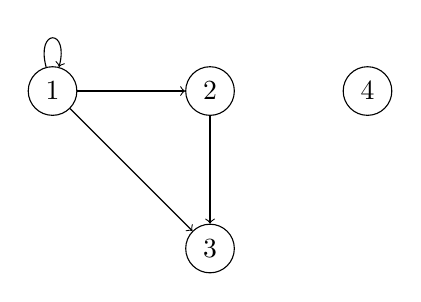
\begin{tikzpicture}[->,node distance=2cm]
  \node[draw,circle] (A) {$1$};
  \node[draw,circle] (B) [right of=A] {$2$};
  \node[draw,circle] (C) [below of=B] {$3$};
  \node[draw,circle] (D) [right of=B] {$4$};
  \draw (A) to [loop above]  (A);
  \draw (A) to  (B);
  \draw (A) to  (C);
  \draw (B) to  (C);
  \end{tikzpicture}
\intertext{हा आलेख $V' = \{1, 2, 3\}$ असणाऱ्या $\tuple{V', E}$ या
  आलेखापेक्षा वेगळा आहे; तो असा दिसतो:}
& 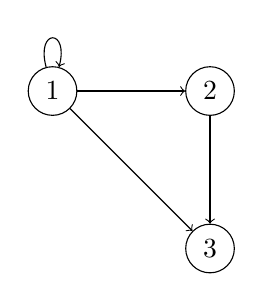
\begin{tikzpicture}[->,node distance=2cm]
  \node[draw,circle] (A) {$1$};
  \node[draw,circle] (B) [right of=A] {$2$};
  \node[draw,circle] (C) [below of=B] {$3$};
  \draw (A) to [loop above]  (A);
  \draw (A) to  (B);
  \draw (A) to  (C);
  \draw (B) to  (C);
  \end{tikzpicture}
\end{align*}
\end{ex}

\begin{prob}
  $\{1, 2, 3, 4\}$ या संचावरील लहान-किंवा-समान असण्याचा $\le$ संबंध
  आलेख म्हणून पाहा आणि त्याची आकृती काढा.
\end{prob}











\section{वृक्ष}\label{sfr:rel:tre:sec}

तर्कशास्त्राच्या सर्व शाखांत महत्त्वाची भूमिका बजावणारा अंशतः क्रमाचा
एक विशिष्ट प्रकार म्हणजे \emph{वृक्ष}. तर्कशास्त्राच्या प्राथमिक भागांत
सांत वृक्ष येतात: उदाहरणार्थ, सूत्रे विन्यासवृक्षात विभागून
समजून घेता येतात, आणि अनेक निष्पत्ती पद्धतींतील
निष्पत्ती सुद्धा सांत वृक्षांच्या स्वरूपात असतात.

विधानीय आणि प्रथमस्तरीय तर्कशास्त्राच्या परिपूर्णता प्रमेयांच्या सिद्धतेतच
अनंत वृक्ष येऊ लागतात; पुढे संपूर्ण गणिती तर्कशास्त्रात त्यांचा वापर होतो.

वृक्षाची संचसैद्धान्तिक संकल्पना आणि आलेख सिद्धांतातील वृक्षाची संकल्पना
यांचा निकटचा संबंध आहे. एका सांत वृक्षाचे चित्र असे आहे:

\begin{center}
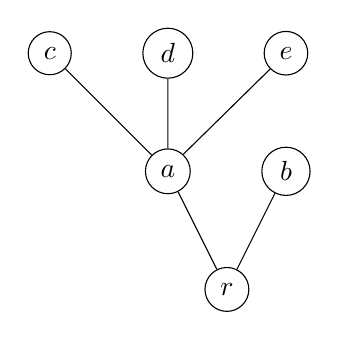
\begin{tikzpicture}[nodes={draw, circle}, -]
\node{$r$} [grow'=up]
    child { node {$a$}
        child { node {$c$} }
        child { node {$d$} }
        child { node {$e$} }
    }
    child { node {$b$} };
\end{tikzpicture}
\end{center}

सर्वांत खालचे $r$ हे शिखर मूळ आहे. $r$ व्यतिरिक्त प्रत्येक शिखराच्या
लगेच खाली नेमके एक पालक शिखर आहे. $x$ पासून कडांवरून वर जात $y$ पर्यंत
पोहोचता येत असेल, तर $x$ चा $y$ शी असणारा संबंध म्हणजे $x$ हा $y$ चा
\emph{पूर्वज} असणे, असे समजू शकतो.

वृक्षातील पूर्वज संबंध हा काटेकोर अंशतः क्रम असतो. यावरून संचसैद्धान्तिक
व्याख्या सुचते. ती मांडण्यासाठी दोन संकल्पना लागतात. $\le$ ने अंशतः
क्रमित केलेल्या $A$ या संचातील \emph{लघुतम घटक} म्हणजे असा
घटक $x \in A$ की सर्व $y \in A$ साठी $x \le y$ असते.
एखाद्या संचाच्या प्रत्येक अरिक्त उपसंचात लघुतम घटक असेल, तर तो संच
$\le$ ने \emph{सुक्रमित} आहे असे म्हणतात.

\begin{defn}[वृक्ष]
\emph{वृक्ष} म्हणजे $T = \tuple{A, \le}$ अशी जोडी की $A$ हा संच असतो,
$\le$ हा $A$ वरील अंशतः क्रम असतो, त्याचा $r \in A$ हा एकमेव लघुतम
घटक असतो (त्याला \emph{मूळ} म्हणतात), आणि सर्व $x \in A$ साठी
$\Setabs{y}{y \le x}$ हा संच $\le$ ने सुक्रमित असतो.
\end{defn}

\begin{defn}[उत्तरवर्ती]
$T = \tuple{A, \le}$ हा वृक्ष आहे असे समजा.
$x,y \in A$, $x < y$ असतील आणि $x < z < y$ असा कोणताही $z \in A$
नसेल, तर $y$ हा $x$ चा \emph{उत्तरवर्ती} आहे असे म्हणतो.
\end{defn}

$x \in A$ च्या उत्तरवर्तींना त्याची \emph{अपत्ये} असेही म्हणतात.
$y$ हा $x$ चा उत्तरवर्ती असेल, तर $x$ ला $y$ चा \emph{पूर्ववर्ती}
किंवा \emph{पालक} म्हणतो.

\begin{prop}
$\tuple{A,\le}$ हा वृक्ष असेल, तर मूळ वगळता प्रत्येक $x \in A$ ला
जास्तीत जास्त एक पूर्ववर्ती असतो.
\end{prop}

\begin{proof}
  $y_1 < x$, $y_2 < x$ आणि $y_1 \neq y_2$ असे समजा. मग
  $\{y_1, y_2\} \subseteq \Setabs{z}{z<x}$. $\Setabs{z}{z<x}$ हा संच
  $\le$ ने सुक्रमित असल्याने त्याच्या $\{y_1, y_2\}$ या उपसंचाला लघुतम
  घटक असतो. तो स्पष्टपणे $y_1$ किंवा $y_2$ असला पाहिजे. म्हणून
  $y_1 \le y_2$ किंवा $y_2 \le y_1$. आपण $y_1 \neq y_2$ गृहीत धरले,
  म्हणून प्रत्यक्षात $y_1 < y_2$ किंवा $y_2 < y_1$. शिवाय,
  $y_1 < x$ आणि $y_2 < x$ या गृहीतकांमुळे $y_1 < y_2 < x$ किंवा
  $y_2 < y_1 < x$. म्हणून $y_1$ आणि $y_2$ हे दोघेही $x$ चे पूर्ववर्ती
  असू शकत नाहीत.
\end{proof}

\begin{defn}
$T = \tuple{A, \le}$ या वृक्षातील $A$ हा अनंत संच असेल, तर वृक्षाला
\emph{अनंत}, आणि अन्यथा \emph{सांत} म्हणतात. $T$ मधील प्रत्येक
$x \in A$ ला फक्त सांत संख्येने उत्तरवर्ती असतील, तर $T$ ला
\emph{सांत शाखनाचा} वृक्ष म्हणतात.
\end{defn}

\begin{defn}[शाखा]
$T = \tuple{A, \le}$ हा वृक्ष दिला असता, $T$ ची \emph{शाखा} म्हणजे
$T$ मधील अधिकतम शृंखला; म्हणजे $B \subseteq A$ असा संच की कोणत्याही
$x, y \in B$ साठी $x \le y$ किंवा $y \le x$ असते, आणि प्रत्येक
$z \in X \setminus B$ साठी असा $u \in B$ असतो की $z \le u$ आणि
$u \le z$ दोन्ही असत्य असतात.

$T$ च्या सर्व शाखांचा संच दर्शवण्यासाठी आपण $[T]$ वापरतो.
\end{defn}

\begin{ex}
सांत शाखनाच्या वृक्षाचे एक प्रसिद्ध उदाहरण म्हणजे $0$ आणि $1$ यांच्या
सांत अनुक्रमांचा \emph{अनंत द्विमान वृक्ष}. त्याला कधी $\{0,1\}^*$ किंवा
$\Bin^*$ असे लिहितात आणि विस्तार संबंध $\sqsubseteq$ ने क्रमित करतात
(उदा., $101 \sqsubseteq 101101$). कोणत्याही द्विमान चिन्हमालेच्या शेवटी
$0$ किंवा $1$ जोडून तिचा विस्तार नेहमी करता येतो. म्हणून या वृक्षात
अनंत घटक असतात: प्रत्येक $s$ या घटकाला नेमके दोन उत्तरवर्ती, $s0$ आणि
$s1$, असतात. त्याचे मूळ म्हणजे $\emptyseq$ हा रिक्त अनुक्रम.
\end{ex}

\begin{ex}
थोडे अधिक सर्वसाधारण उदाहरण म्हणजे नैसर्गिक संख्यांच्या सांत अनुक्रमांचा
$\Nat^*$ हा संच आणि त्यावरील विस्तार संबंध $\sqsubseteq$; हाही वृक्ष
असतो. तो स्पष्टपणे सांत शाखनाचा नाही: प्रत्येक $s \in \Nat^*$ ला अनंत
उत्तरवर्ती $sn$ असतात, प्रत्येक $n \in \Nat$ साठी एक. $\sqsubseteq$
नुसार बंद असलेला प्रत्येक $A \subseteq \Nat^*$ हा $\Nat^*$ चा
\emph{उपवृक्ष} असतो. (म्हणजे $A$ असा आहे की $s \in A$ आणि
$s' \sqsubseteq s$ असतील, तर $s' \in A$ सुद्धा.) सर्व सांत वृक्ष
$\Nat^*$ चे सांत उपवृक्ष म्हणून दर्शवता येतात.
\end{ex}

\begin{prop}[K\H{o}nig यांचे उपप्रमेय]
$T = \tuple{A,\le}$ हा सांत शाखनाचा अनंत वृक्ष असेल, तर $T$ ला
एक अनंत शाखा असते.
\end{prop}

संगणनीयता सिद्धांतात वारंवार वापरले जाणारे K\H{o}nig यांच्या उपप्रमेयाचे
एक विशेष रूप, ज्याला \emph{दुर्बल K\H{o}nig उपप्रमेय} म्हणतात, असे आहे:
$\{0,1\}^*$ च्या प्रत्येक अनंत उपवृक्षाला एक अनंत शाखा असते.











\section{संबंधांवरील क्रिया}\label{sfr:rel:ops:sec}

संबंधांत बदल करणे किंवा त्यांना एकत्र करणे अनेकदा उपयोगी पडते.
\ref{sfr:rel:ord:prop:stricttopartial} मध्ये आपण संबंधांचा
\emph{संयोग} पाहिला; तो म्हणजे दोन संबंधांकडे जोड्यांचे संच म्हणून
पाहिल्यावर त्यांचा संयोग. त्याचप्रमाणे,
\ref{sfr:rel:ord:prop:partialtostrict} मध्ये संबंधांचा सापेक्ष फरक
पाहिला. संबंधांवर करता येणाऱ्या आणखी काही क्रिया पुढीलप्रमाणे आहेत.

\begin{defn}\label{sfr:rel:ops:relationoperations}
$R$, $S$ हे संबंध आणि $A$ हा कोणताही संच असू द्या.

$R$ चा \emph{व्युत्क्रम} म्हणजे $R^{-1} = \Setabs{\tuple{y, x}}{\tuple{x,
    y} \in R}$.

$R$ आणि $S$ यांचा \emph{सापेक्ष गुणाकार} म्हणजे $(R \mid S) =
\{\tuple{x, z} : \exists y(Rxy \land Syz)\}$.

$R$ चे $A$ वरील \emph{मर्यादन} म्हणजे $\funrestrictionto{R}{A}= R
\cap A^2$.

$R$ चा $A$ वर \emph{प्रयोग} म्हणजे $\funimage{R}{A} = \{y :
(\exists x \in A)Rxy\}$
\end{defn}

\begin{ex}
$S \subseteq \Int^2$ हा $\Int$ वरील उत्तरवर्ती संबंध असू द्या, म्हणजे
$S = \Setabs{\tuple{x, y} \in \Int^2}{x + 1 = y}$; त्यामुळे $Sxy$
तेव्हा आणि केवळ तेव्हाच, जेव्हा $x + 1 = y$.

$S^{-1}$ हा $\Int$ वरील पूर्ववर्ती संबंध आहे, म्हणजे
$\Setabs{\tuple{x,y}\in\Int^2}{x -1 =y}$.

$S\mid S$ म्हणजे
$ \Setabs{\tuple{x,y}\in\Int^2}{x + 2 =y}$

$\funrestrictionto{S}{\Nat}$ हा $\Nat$ वरील उत्तरवर्ती संबंध आहे.

$\funimage{S}{\{1,2,3\}}$ म्हणजे $\{2, 3, 4\}$.
\end{ex}

\begin{defn}[संक्रमक संवरण] $R \subseteq A^2$ हा द्विपदी संबंध असू द्या.

$R$ चे \emph{संक्रमक संवरण} म्हणजे $R^+ = \bigcup_{0 < n \in
\Nat} R^n$, जेथे $R^1 = R$ आणि $R^{n+1} = R^n \mid R$ अशी पुनरावर्ती
व्याख्या करतो.

$R$ चे \emph{परावर्ती संक्रमक संवरण} म्हणजे $R^* = R^+ \cup \Id{A}$.
\end{defn}

\begin{ex}
$S \subseteq \Int^2$ हा उत्तरवर्ती संबंध घ्या. $S^2xy$ तेव्हा आणि केवळ
तेव्हाच, जेव्हा $x + 2 = y$; $S^3xy$ तेव्हा आणि केवळ तेव्हाच, जेव्हा
$x + 3 = y$; इत्यादी. म्हणून $S^+xy$ तेव्हा आणि केवळ तेव्हाच, जेव्हा
एखाद्या $n \geq 1$ साठी $x + n = y$. दुसऱ्या शब्दांत, $S^+xy$ तेव्हा
आणि केवळ तेव्हाच, जेव्हा $x < y$; आणि $S^*xy$ तेव्हा आणि केवळ तेव्हाच,
जेव्हा $x \le y$.
\end{ex}

\begin{prob}
$R$ चे संक्रमक संवरण खरोखर संक्रमक आहे, हे दाखवा.
\end{prob}


